\documentclass[table]{elegantpaper}
\usepackage{datetime2}
\usepackage[T1]{fontenc}
\usepackage{graphicx}
\usepackage{listings}
\usepackage{listings-rust}
\usepackage{pgf-pie}
\usepackage{rotating}
\usepackage{tabularray}
\usepackage{tabularx}

\DTMusemodule{english}{en-GB}
\DTMnewdatestyle{short}{
  \renewcommand{\DTMdisplaydate}[4]{
    \DTMenglishmonthname{##2} \number##1\relax
  }
  \renewcommand{\DTMDisplaydate}{\DTMdisplaydate}
}
\newcommand{\shorttoday}{{\DTMsetdatestyle{short}\today}}
\renewcommand{\updatetext}{}

\graphicspath{{./images/}}
\DeclareEmphSequence{\bfseries,\itshape,\upshape}
\lstset{xleftmargin=\parindent,xrightmargin=\parindent}

\title{OlaVM: An Ethereum compatible ZKVM}
\author{Sin7Y, Applied R\&D Team\thanks{\url{https://twitter.com/Sin7Y_Labs}}}
\date{\shorttoday}

\addbibresource[location=local]{reference.bib}

\begin{document}
    \maketitle
    \begin{abstract} 

    \noindent We are developing a ZK-ZKVM platform for Ethereum\cite{website:Ethereum} that will offer the following features: 
    (1) Programmable Privacy: unlike specific privacy, Ola could private for everything which supports user-defined functions; 
    (2) Optional Privacy: both the project side and user side could optionally choose to deploy/send public/private type; 
    (3) Compliance-friendly Privacy: Through the means of viewing keys that can be shared with third parties, we create a compliance-friendly landscape, providing the possibility for 
    regulators to track the private assets, avoiding the disadvantages of untraceable assets, such as Tornado Cash\cite{website:Tornado-cash}; 
    (4) High Programmability: a customize GPL language which has more advanced features and is more programmable than DSL\cite{website:DSL}; 
    (5) High Performance: customize full-featured zk-friendly ZKVM, OlaVM\cite{website:OlaVM}, can quickly execute transactions and generate proofs; 
    (6) Developer-friendly language: Ola-lang\cite{website:Ola-lang}  is customized for smart contract development with syntax similar to Rust, making it convenient for developers quickly adopt it; 
    (7) Developer-friendly IDE: Ola-lang language is integrated into the Visual Studio Code, making it convenient for traditional developers to start building;
    (8) Better Scalability: based on the LLVM compilation framework, it is easier to achieve compatibility with other advanced programming languages; 
    (9) Uptable view key: avoiding third-party continuous monitoring and tracking of an account's status; 
    (10) Data ownership: taking the control of their asset information and on-chain data.
    \\ \hspace*{\fill} \\
    \noindent Ola is a rapidly developing project and this is the second whitepaper that will describe the design philosophy and specifications of our full-featured zk-friendly ZKVM,  
    OlaVM\cite{website:OlaVM} and developer-friendly general purpose smart contract language, Ola-lang\cite{website:Ola-lang} detailedly. Implementation details related to privacy will be released in the upcoming third whitepaper upon releasing the test net.
    \\ \hspace*{\fill} \\
    \noindent \textbf{Key words: Privacy, Programmability, ZKVM, Smart Contract, Data Ownership.}    
\end{abstract}
    \tableofcontents
    \section{Introduction}\label{sec:introduction}

In the past few years, we have witnessed a rapid development of the blockchain industry, influx of capital, users, and builders has enabled unprecedented growth and potential of the entire industry. However, blockchain is still somewhat in its infancy, infrastructure is still maturing. One of the largest challenges is the low transactional throughput of public blockchain systems, especially the largest public programmable blockchain Ethereum \cite{website:Ethereum}, which in the best case scenario \cite{website:Etherscan-chart}, processes up to 23 transactions per second, far less than traditional centralized systems. 

There are many reasons for the congestion of the Ethereum network, such as the POW \cite{website:POW} consensus algorithm (The Merge upgrade \cite{website:The-Merge} to POS \cite{website:POS} consensus now), the repeated execution of verification process of all transactions by nodes, and the serial execution of transactions; for the above reasons, many projects are trying to scale Ethereum through different means. Approach 1: Launching new public blockchains, independent of Ethereum, using faster consensus algorithms or faster transaction execution to achieve higher TPS, such as BSC \cite{website:BSC}, Solana \cite{website:Solana}, Aptos \cite{website:Aptos}, etc; Approach 2: Ethereum Sidechain, using faster consensus algorithms and then regularly synchronizing to Ethereum, such as Polygon \cite{website:Polygon}, Optimism \cite{website:Optimism}, Arbitrum \cite{website:Arbitrum}, etc; Approach 3: ZK(E)VM, a Layer2 network of Ethereum, using ZK technology to solve the problem of repeated execution of transactions, such as Polygon Hermez \cite{website:Polygon-Hermez}, Zksync \cite{website:Zksync} etc.

Scaling is not the only problem that has to be solved in the long term for Ethereum and the wider blockchain space. There are many excellent teams working rigorously on scaling solutions, the ola team believe that the next crucial feature to be implemented is privacy. Blockchains being a public ledger, all transactions taking place on-chain, meaning state changes containing the asset information related to an address or account is open and transparent. 

Excessive information transparency leads to: 

\begin{enumerate}
    \item MEV (Maximal Extractable Value) issues. Miners can selectively package transactions based on its fee, resulting in transactions with lower fees having a lower likelihood of being processed, if ever, forcing users to increase their fees. More concerning:
    \item Front running and censorship attacks, through the means of MEV. Block producers in programmable blockchains can use MEV to exploit certain smart contracts deployed on the blockchain (Such as DEXes and other DeFi products). They may also censor certain addresses. Such an attack could be that the miner or block producer sees a buy order in the memory pool (where transactions that are not yet appended to the blockchain are stored) and adds their own buy order on that particular DEX, thus increasing the price of the given token. The other transaction that is added is a sell order of given token and the third order is the buy order of the third party for the new increased price. Resulting in huge security issues and in the past year hackers have managed to steal assets roughly amounting to 2 billion dollars.
    \item User data ownership problems, both the assets information and transaction information of addresses are open to being monitored and used, which is contrary to the vision of Web3 \cite{website:Web3}. Therefore, when the scaling problem is solved, privacy will become the next urgent feature to achieve. In the world of blockchain, privacy is not a new topic, it has long been studied and supported by the Zcash team \cite{website:Zcash}.
\end{enumerate}

\subsection{Non Programmable Privacy}

In addition to the Zcash team, other public blockchains that implement private transactions include Monero \cite{website:Monero}, Dash \cite{website:Dash}, Grin \cite{website:Grin}, and others. However, these public chains lack programmability and can only be used for simple private transfer of assets. Consequently, their ecosystem development lags far behind Ethereum, which has become the largest public chain in the ecosystem due to its programmability, but Ethereum lacks privacy features.

Therefore, some projects have begun to explore ways to introduce privacy to Ethereum, such as the ZK-ZKRollup application zk.money \cite{website:zk.money} developed by the Aztec \cite{website:Aztec} team. However, the current zk.money product has been discontinued, mainly because it's privacy features only apply to simple single transfer scenarios. Given the current explosion of Defi applications, asset transfer is only one of the simplest financial scenarios, and therefore the user base is limited, while the maintenance costs continue to accrue.
\begin{figure}[!ht]
    \centering
    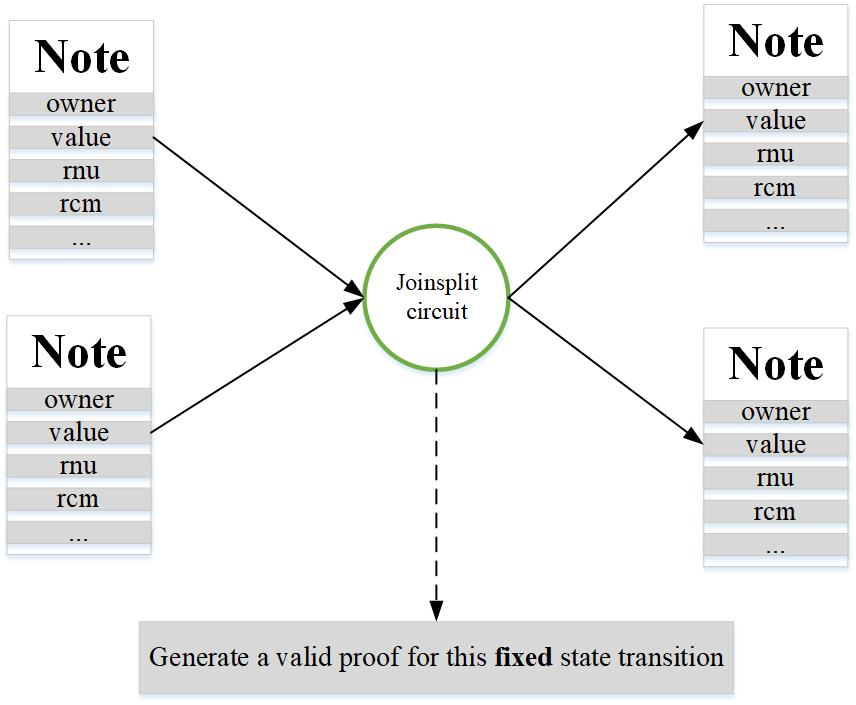
\includegraphics[width=0.4\textwidth]{Example of Non Programmable privacy.jpg}
    \caption{Example of Non Programmable Privacy}
    \label{fig:Example of Non Programmable Privacy}
\end{figure}

\figref{fig:Example of Non Programmable privacy} shows the simple logic of non programmable privacy. The value change logic corresponding to the input and output notes in Section \ref{section: sending-notes} are also fixed, generally in the form of ``A + B = C + D''. Manta Network \cite{website:Manta-network} is a public blockchain that supports user-defined token privacy transfers, and the privacy transaction 
constraint circuits of all fungible tokens can be used to reuse the above logic.

A ZK-ZKRollup application of a single scenario use case, is similar to a ZKRollup application of a single scenario use case. If you want to use the asset in other applications or for other use cases, you must cross the asset to another application through a bridge, which brings with it very poor user experience. Therefore, just as ZKRollups need to 
transition to ZK(E)VMs, ZK-ZKRollup also need to transition to ZK-ZKVMs (Appendix \ref{section: solidity-compatibility} explains how to get solidity compatibility).

\subsection{Programmable Privacy}

ZK-ZKVM has two main features (1) It's a privacy-first platform, not privacy-only. This means that users can choose the transaction type, public or private, depending on their need. Just similar to the Zcash;
(2) Programmability, you can deploy any smart contract, public or private, depending on the needs of the project side. Compared with non programmable privacy, the main difference is the logic of state transition in a note \ref{section: sending-notes}, \figref{fig:Difference between Non Programmable Privacy and Programmable Privacy} simply shows the difference 

\begin{figure}[!ht]
    \centering
    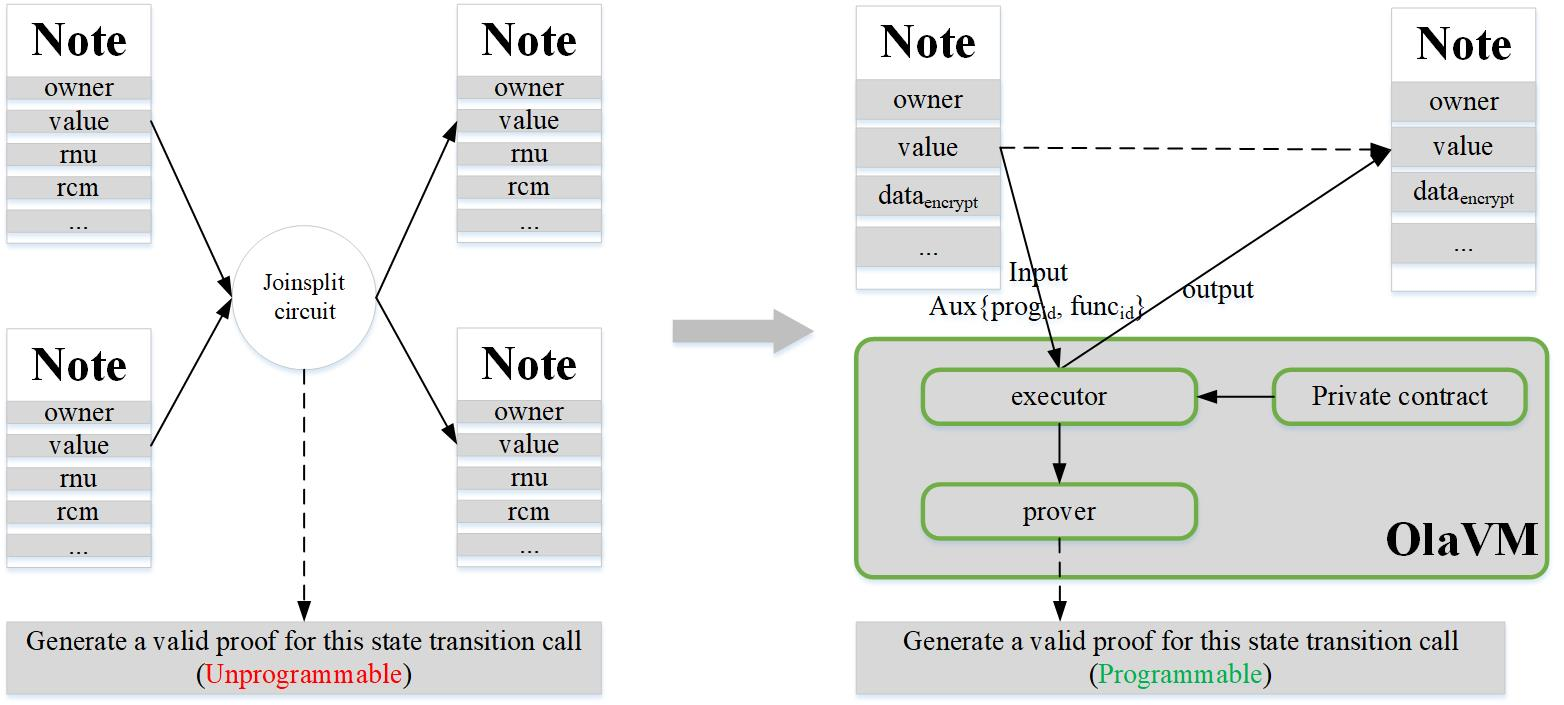
\includegraphics[width=0.6\textwidth]{Difference between Non Programmable Privacy and Programmable Privacy.jpg}
    \caption{Difference between Non Programmable Privacy and Programmable Privacy}
    \label{fig:Difference between Non Programmable Privacy and Programmable Privacy}
\end{figure}

The current projects focusing on programmable privacy are Aleo \cite{website:Aleo} and Aztec. Aleo is a 
privacy-first public blockchain, from Bitcoin \cite{website:BTC} to Ethereum to Zcash \cite{website:Zcash} to Aleo. It brings the public blockchain into a new era,
supporting programmable privacy. 
It has reached the testnet stage and supports developers to deploy privacy contracts on it; 
Aztec focuses on doing Layer2 programmable privacy for Ethereum, a project 
called Aztec3 \cite{website:Aztec3}, is still in development.

Before we clarify the different approaches to get programmability, we should give some explanations on Domain Specific Language (DSL) and General Purpose Language (GPL) \cite{website:DSL}.
DSL is defined as a computer programming language of limited expressiveness focused on a particular domain, limited expressiveness means it just supports a bare minimum of features 
needed to support its domain. You can't build an entire software system in a DSL; rather, you use a DSL for one particular aspect of a system. While GPL is defined as a general-purpose programming language

So there are often two ways to achieve programmability, one is to design a DSL, such as Circom \cite{website:Circom}, Pil \cite{website:Pil}, Noir \cite{website:Noir}, etc; the other is SCL, 
such as Cairo1.0 \cite{website:Cairo1.0}, Solidity \cite{website:Solidity}, Ola lang \cite{website:Ola-lang} and so on. As we have mentioned before, the main difference is that SCL supports more complex structures and has 
higher abstraction, it's more suitable for writing complex business logic and meanwhile, and DSL is more suitable for some simple computational expressions. 
Take Pil \cite{website:Pil} language as an example, you can directly use it to define a simple micro-op, such as ``A * B + C'', or ``A * B * C + D'' and other simple combinations. 
\tabref{table:Difference between DSL and SCL} briefly shows some of the differences between DSL and SCL.

\begin{table}[!ht]
    \centering
    \begin{tabular}{|c|c|c|c|c|c|}
        \hline
        \emph{Type} & \emph{Abstraction} & \emph{Process} & \emph{Difficulty} & \emph{Examples} & \emph{Notes} \\ 
        \hline
        DSL & low & program -> arith-ops -> ops gadgets & normal & \makecell{circom \\ noir \\ cairo} & \makecell{1. semantic analysis \\ 2. codeGen optimization} \\
        \hline
        \makecell{SCL \\ (ISA/VM)} & high & program -> bytecodes -> cpu circuit & hard & \makecell{solidity \\ cairo1.0 \\ ola lang} & \makecell{1. need a compiler \\2. re-use LLVM framework} \\
        \hline
    \end{tabular}
    \caption{Difference between DSL and SCL}
    \label{table:Difference between DSL and SCL}
\end{table}

If you want to prove a program written by DSL is executed correctly (this is what ZKDSL means), you may need to predefine some common operators, each of them corresponding to a circuit, called a gadget \cite{website:Gadget}. 
Developers can use these operators to implement desired functions, but it's difficult to handle the call and return logic between functions. Meanwhile, If you want to prove a program written by SCL is executed correctly (this is what ZKVM means), 
 you need to design corresponding constraints for each instruction, collectively referred to as CPU circuit; therefore, Any program will be compiled into 
 bytecodes composed of these instructions, and then constrained by the CPU circuit.

Ola achieved a customized SCL to get programmability even though it's harder to implement than DSL, because we could get benefits from it as follows:
 \begin{itemize}
 \item A higher abstraction and programmable language, allowing developers to write smart contracts with arbitrary logic;
 \item A full-featured zk-friendly VM can be designed to achieve higher system performance;
 \item LLVM-based compiler can be more easily compatible with other advanced programming languages.
\end{itemize}

\subsection{Full-featured ZK-friendly ZKVM}

As mentioned earlier, the best way to achieve programmability is to design a ZKVM with a custom Instruction Set Architecture, a custom smart contract language, and a custom compilation, etc. 
ZKVM is a virtual machine that can execute any program and at the same time generate a zero-knowledge proof of the correctness of the execution process. Therefore, the speed of proof generation 
is very critical, and it will directly affect the performance of the entire system.

The key to obtaining a full-featured zk-friendly ZKVM is how to obtain(1)the smallest execution trajectory; (2)the most concise state transition constraint logic; (3)the fastest 
zero-knowledge proof algorithm. The smallest execution trajectory means: for the same computational logic, OlaVM \cite{website:OlaVM} can be expressed with the least instructions, the main technical means are the 
support for non-deterministic computation at the computational level, and the register-based design is used at the memory access level; The most concise state transition constraint logic means: 
for the same computational logic, OlaVM \cite{website:OlaVM} can constrain the entire execution trajectory with the least polynomials and the smallest order. The main means is to obtain the instruction with the least 
number of instructions through the Algebraic RISC architecture. The number of Instruction Set Architecture determines the complexity of Cpu constraints; faster zero-knowledge proof algorithm 
Meaning: For the same calculation, OlaVM \cite{website:OlaVM} can complete the proof generation process in less time, which mainly depends on the Godilocks \cite{website:Goldilocks} field, a finite field less than 64bit, compared to the 
SNARK system based on large bit width elements of elliptic curves, based on The STARK algorithm of the Goldilocks \cite{website:Goldilocks} field can be executed faster.

Subsequent chapters will explain in detail Ola's design philosophy and design specifications for obtaining a Full-featured ZK-friendly ZKVM. As the first programmable privacy layer network 
based on ZKVM, Ola will support the following scenarios for different subjects:

\begin{itemize}
\item For Developers
    \begin{itemize}
    \item Developers can freely choose to deploy public contracts(Account-based), privacy contracts(Note-based), and ordinary contracts(Account and Note-based)
        \begin{enumerate}
        \item For public contracts, Ola functions as a ZKVM;
        \item For privacy contracts, Ola functions as a ZK-ZKVM;
        \item For ordinary contracts, Ola functions as a ZK-ZKVM or ZKVM, depending on the user's transaction type;
        \end{enumerate}
    \item Transfer of assets between public and private accounts
    \item Intra-contract, no bridge contract is required, supported by default;
    \item Cross-contract, a bridge contract is required;
    \end{itemize}
\item For Users
    \begin{itemize}
    \item For ordinary contract types, users can freely choose the transaction type;
    \item For public/private contract types, users can only execute transactions of the corresponding type;
    \item Users have a view key to disclose executed private transactions;
    \item Ola supports the update of the view key so that after the view key is exposed, the privacy transactions executed by the user in the future will always be parsed;
    \item Ola supports asset transfers between public and private accounts;
    \end{itemize}
\end{itemize}
\subsection{Outline}

Ola is a full stack developer framework for zero-knowledge applications, the whole framework is shown as \figref{fig:Ola framework}:
\begin{figure}[!ht]
    \centering
    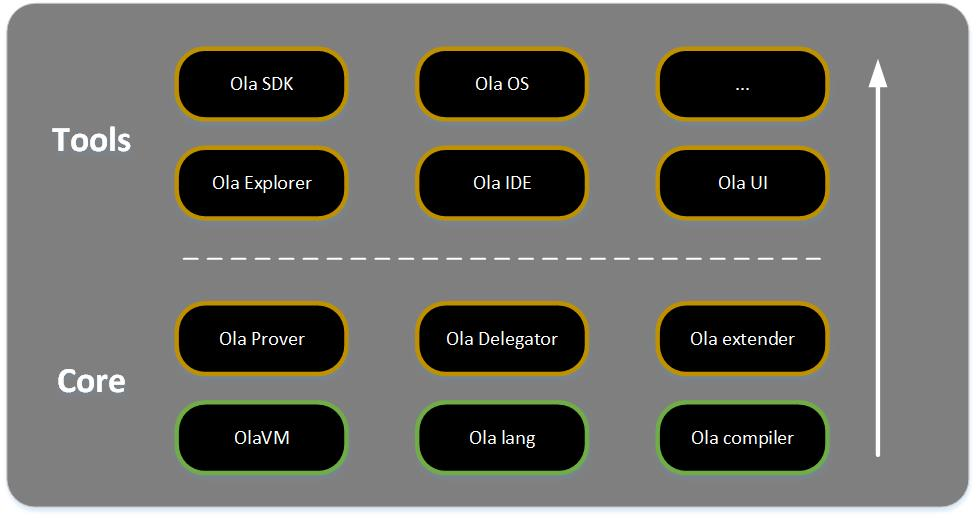
\includegraphics[width=0.6\textwidth]{vm/Ola framework.jpg}
    \caption{Ola framework}
    \label{fig:Ola framework}
\end{figure}

The green borders refers to the modules we have completed implementation, and others stand for the modules we will implement in the future. In the remaining sections of this whitepaper, we will introduce those modules 
as follows:
\begin{itemize}
    \item Section \ref{sec:olavm-a-full-featured-zk-friendly-zkvm} mainly describes the design of Ola's virtual machine, including our zk-friendly design schemes;
    \item Section \ref{sec:ola-lang} mainly describes the design of the customized smart contract language, Ola-lang and the framework of Ola compiler based LLVM;
    \item Section \ref{sec:ola-compiler} mainly describes the design of Ola compiler;
    \item Section \ref{sec:zk-zkvm} mainly describes key points on achieving privacy;
    \item Section \ref{sec:algorithms} mainly describes algorithms used in Ola, including zk and hardware acceleration algorithms;
    \item Section \ref{section:appendix} mainly describes the key features we researched to be supported in the future and our frameworks around that;
    \item Section \ref{sec:glossary} mainly describes some basic notations;
\end{itemize}


    \section{ZK-ZKVM} \label{sec:zkzkvm}

OlaVM \ref{section: olavm} is a ZK-VM which is a system that uses zk technology to implement a verifiable circuit system for general computation. However, it has some issues where privacy is required, for example, quotation data of commercial competition, anonymous auction, etc. The ZK-VM's each proof generation leaks the witness data, such as the name and function of the called contract, parameters, and so on.

To address this privacy concern, the ZK-ZKVM system has been developed. This system builds on top of ZK-VM but adds an extra layer of privacy by ensuring that all witness data is private and does not reveal any information. This is achieved through the use of different permissioned private key systems and a note mechanism similar to ZCash's UTXO model.

The core technology of ZK-ZKVM is the use of different permissioned private key systems. These keys are used to encrypt and decrypt the witness data, ensuring that it remains private and secure. Additionally, the note mechanism is used to further enhance the privacy of the system. Each note represents a commitment to a certain amount of value, and it is impossible to deduce any information about the transaction from this commitment.

The importance of ZK-ZKVM lies in its ability to address the privacy concerns that exist in ZK-VM. With ZK-ZKVM, users can conduct transactions on public blockchains with the assurance that their sensitive information is secure and private. This makes it suitable for a wide range of use cases that require high levels of privacy, such as financial transactions or data sharing.

Furthermore, ZK-ZKVM also offers the same scalability benefits as ZK-VM. By allowing for off-chain computation and verification, it reduces the burden on the main blockchain and increases transaction throughput. This makes it a more efficient and effective solution for blockchain scaling than traditional solutions.

In Section \ref{section: zkzkvm-framework} we explain our basic framework of ZK-ZKVM. Then, in Section \ref{section: zkzkvm-key}, we explain the key system design in our ZK-ZKVM system. Then, in Section \ref{section: zkzkvm-note}, we explain the note design in our ZK-ZKVM system. Then, in Section \ref{section: zkzkvm-user-end-prove} and \ref{section: zkzkvm-delegable-prove}, we compare two different proof generation schemes.

\subsection{Framework}\label{section: zkzkvm-framework}
\subsection{Key}\label{section: zkzkvm-key}
\subsection{Note}\label{section: zkzkvm-note}
\subsection{User End Prove}\label{section: zkzkvm-user-end-prove}
\subsection{Delegable Prove}\label{section: zkzkvm-delegable-prove}
    \section{Ola-Lang: Dev-friendly SM language}\label{sec:Ola-Lang}

Ola is a high-level programming language for developing OlaVM smart contracts.
It is Turing complete and can be used to write arithmetic programs.

The computing process is proven by the OlaVM back-end proof system, which verifies that the OlaVM processing is accurate.

Most of the existing programming languages in the ZKP field require fundamental knowledge of the circuit field,
which is not universal, or the execution process is difficult to be proven and verified by ZKP.

\subsection{Language introduction}\label{section: ola-lang-language-introduction}
\subsection{Language Elements}\label{section: ola-lang-language-elements}


\subsubsection{Variables}

\subsubsection*{Identifier}

Variables consist of numbers (\texttt{0-9}), ASCII uppercase and lowercase letters (\texttt{a-zA-Z}), underscores (\texttt{\_}).
Variables cannot start with a number.

\begin{lstlisting}
fn foo() {
    // declare and ine `_variable`
    u32 _aBC123 = 2;   // identifiers start with "_"
    // u32 0a = 2;  define error, identifiers can't start with number
}
\end{lstlisting}

\subsubsection*{Declaration}

Variables need to be declared in order to be used. To avoid variables being undefined, it needs to be initialized at declaration time. 

\begin{lstlisting}
fn foo() {
    // declare and define `a`
    u32 a = 2;
    // redefine `a`
    a = 3;
}
\end{lstlisting}

\subsubsection*{Scope}

For security reasons, variable definitions do not support Shadowing. 
If you need multiple adjacent variables with similar logical meanings, use a variable or type suffix.

\begin{lstlisting}
fn foo() {
    u32 a = 5;
    {        
        u32 a = 25; // compile error: redeclared variable 'a'
    };    
    u32 a = 25; // compile error: redeclared variable 'a'

    a = 25; // ok
}
\end{lstlisting}

Variables differ from constants in that the scope of a variable is limited to the current function itself and global variables are not supported.

\begin{lstlisting}
fn foo() -> u32 {
    // return a; <- not allowed
    return 2;
}

fn bar() -> u32 {
    32 a = 2;
    return foo();
}
\end{lstlisting}

Variables in a \texttt{For-Loop} loop are scoped only inside the loop.

\begin{lstlisting}
fn foo() -> u32 {
    u32 a = 0;
    for (u32 i = 0; i < 5; i++) {
        a = a + i;
    }
    // return i; <- not allowed
    return a;
}
\end{lstlisting}

\subsubsection{Data Type}

Ola is a statically typed language, and variable types must be known at compile time to avoid most runtime exceptions. 
Three basic types and multiple complex types are supported.

\subsubsection*{Basic Types}

The basic types include integer and boolean types.

There are several types of integer types: \texttt{u32}, \texttt{u64}, and \texttt{u256}, and currently only u32 operations are supported now. 
All types are built on the basis of the \texttt{field} type.
Ola provides the above-mentioned basic libs of various integer types based on the field implementation, which is convenient for developers to write complex logic.

\begin{lstlisting}
u32 a = 2; // u32
u64 b = 2; // u64
u64 b  = 0xffffl; // u64
u256 d = 102411ll  // u256
\end{lstlisting}

\begin{lstlisting}
bool a = true;
bool b = false;
\end{lstlisting}
\subsubsection*{Arrays}

Ola supports statically typed arrays. The data types of array elements must be consistent, and the array size must be determined at compile time. 

Array elements are numbered from zero and are accessed using \texttt{[index]} for addressing.

Array declarations must be initialized, and the array declaration format is \texttt{type} and \texttt{[] (\texttt{type []})}, and the array size must be specified.
Two ways to initialize arrays are provided:
\begin{itemize}
    \item Split the list of elements by commas, \texttt{[array\_element1,array\_element2,...]}.
    \item Array declaration and initialization with consistent array elements, \texttt{[array\_value; size]}.
\end{itemize}

\begin{lstlisting}
u32[5] a = [1, 2, 3, 4, 5]; 
bool[3] b = [true; 3]; // initialize a bool array with value true
\end{lstlisting}

\subsubsection*{Two-dimensional Arrays}

Two-dimensional arrays are declared and used similarly to one-dimensional arrays, except that the internal elements of a two-dimensional array are also one-dimensional arrays. 

Declare \texttt{type [row\_size][col\_size]}, and initialize \texttt{[[],[],...]}.

\begin{lstlisting}
// Array of two elements of array of 3 elements

u32[2][4] a = [[1, 2, 3, 4],[4, 5, 6, 7]];

u32[4] b = a[1]; // should be [4, 5, 6, 7]
\end{lstlisting}

Array Slicing

Similar to Rust, arrays can be created by slicing an array to copy the generated array,

\begin{lstlisting}
u32[5] a = [1, 2, 3, 4, 5];
u32[3] b = a[2..4];   // initialize an array copying a slice from `a`
// array b is [3, 4, 5]
\end{lstlisting}

\subsubsection*{Tuples}

A collection of elements of two types, with each element in the collection accessed through \texttt{.} (\texttt{t.0}, \texttt{t.1}).

\begin{lstlisting}
fn main() -> bool {
    (u32[2], bool) v = ([1, 2], true);
    v.0 = [2, 3];
    return v.1;
}
\end{lstlisting}

\subsubsection*{Structs}

A combination of multiple data types to form a new custom combination type. Struct members are accessed via \texttt{.} (\texttt{struct\_name.struct\_field})

\begin{lstlisting}
struct Person {
    age: u32,
    id: u64,
}

fn foo() {
   Person person = Person {
        age: 18,
        id: 123456789,
    };
    person.age = 25;
}
\end{lstlisting}

\subsubsection*{Enumerations}

The enumeration type is defined by the keyword \texttt{enum}.

\begin{lstlisting}
contract Foo {
    u256 const x = 56;
    enum ActionChoices {
        GoLeft,
        GoRight,
        GoStraight,
        Sit
    }
    ActionChoices const choices = ActionChoices.GoLeft;
}
\end{lstlisting}


\subsubsection*{Type Alias}

To increase code readability, defining a type alias for each type is supported. At compile time, the type alias will be replaced with real types.

\begin{lstlisting}
type balance = u256;

fn main() -> balance {
    balance a = 32;
    a -= 2;
    return a;
}
\end{lstlisting}

\subsubsection{Constant}

Constants can only be declared as constant expressions when defined with the \texttt{const} keyword.

Compile time determination cannot be redeclared and assigned, that is, once defined, it can only be used within its scope, and it is recommended to declare with all capital letters and \texttt{\_} concatenation. 

\begin{lstlisting}
const u32 ONE = 1;
const u32 TWO = ONE + ONE;

const u32 HASH_SIZE = 256;

fn hash_size() -> u32 {
    return HASH_SIZE;
}
\end{lstlisting}

\subsubsection{Operators}

Provides operators such as arithmetic, logic, relational, bits, and so on. Except for the arithmetic operation acting on numerical values, which is Mod p, all others are standard semantics. 

\subsubsection*{Arithmetic operators}

All arithmetic operators are modulo P(Field element).

Arithmetic operators can be combined with the assignment operator \texttt{=} to form new compound operators \texttt{+=}, \texttt{-=}, \texttt{*=}, \texttt{/=}, \texttt{\%=}, with arithmetic operators having higher priority than compound operators. 

\begin{table}
\centering
\begin{tabular}{c|c|c}
Operat & Example & Explanation \\ \hline
+ & a + b & Arithmetic addition modulo p \\
- & a - b & Arithmetic subtraction modulo p \\
* & a * b & Arithmetic multiplication modulo p \\
/ & a / b & Arithmetic multiplication inverse modulo p \\
\% & a \% b & The modulo of arithmetic integer division \\
** & a ** b & Power modulo p \\
\end{tabular}
\caption{Arithmetic operators}
\end{table}

\subsubsection*{Boolean operators}

Support with AND(\texttt{\&\&}) as well as OR(\texttt{||}), with the latter having higher priority.

\begin{table}
\centering
\begin{tabular}{c|c|c}
Operator & Example & Explanation \\ \hline
\&\& & a \&\& b & Boolean operator and (AND) \\
|| & a || b & Boolean operator or (OR) \\
! & ! a & Boolean operator NEGATION \\
\end{tabular}
\caption{Boolean operators}
\end{table}

\subsubsection*{Relational operators}

The return result of the relational operator is type \texttt{bool}

\begin{table}
\centering
\begin{tabular}{c|c|c}
Operator & Example & Explanation \\ \hline
== & a == b & equal \\
!= & a != b & not equal \\
< & a < b & less than \\
> & a > b & greater than \\
<= & a <= b & less than or equal to \\
>= & a >= b & greater than or equal to \\
\end{tabular}
\caption{Relational operators}
\end{table}

\subsubsection*{Bitwise operators}

All bitwise operators are modulo p, containing bit or and non and shift operations.
\begin{table}
\centering
\begin{tabular}{c|c|c}
    Operator & Example & Explanation \\ \hline
    \& & a \& b & bit and \\
    \textbar{} & a \textbar{} b & bit or \\
    \textasciicircum{} & a \textasciicircum{} b & XOR 32 bits \\
    << & a << 3 & shift left \\
    >> & a >> 3 & shift right \\
    \textasciitilde{} & \textasciitilde{}a & Complement 32  bits \\
\end{tabular}
\caption{Bitwise operators}
\end{table}

Bitwise operators can be combined with the assignment operator \texttt{=} to form the new compound operators \texttt{\&=}, \texttt{\textbar=}, \texttt{\textasciicircum=}, \texttt{<<=}, \texttt{>>=}, 
with bitwise operators taking precedence over compound operators.

\subsubsection{Control Flow}

\subsubsection*{Conditional statement}

Control conditional branch and select different branch programs to execute according to different conditions. 
If the expression value is nonzero, the branch body is executed.
It comes in two forms:

\begin{itemize}
    \item Contains only single branch \verb|if|: \verb|if conditional_expression {statements}|.
    \item Contains multiple branches of \verb|if| and \verb|else|: 
    \verb|if conditional_expression {statements}| \\
    \verb|else {statements}|.

\end{itemize}

\begin{lstlisting}
fn foo(u32 a) -> u32 {
    
    // Similar to rust, the result of a conditional expression 
    // can be received directly by the variable
    u32 b = if (a + 1 == 2) { 1 } else { 3 };
    return b;
}
\end{lstlisting}

Note: Conditional statements support ternary conditional operators.

\begin{lstlisting}
fn foo(u32 a) -> u32 {
    u32 b = a + 1 == 2 ? 1 : 3;
    return b;
}
\end{lstlisting}

\subsubsection*{Loop statement}

Repeats the statement within the loop for a specified number of times based on the loop condition.

\verb|for-loop| statement is supported. Its syntax is \\
\verb|for (init_expression; conditional_expression; loop_expression) {statements}|.

The execution process is:
\begin{enumerate}
    \item Calculate the \verb|init_expression|, namely the loop initialization.
    \item Calculate the \verb|conditional_expression|. If the result is \verb|true|, the loop body \verb|statements| are executed, followed by the \verb|loop_expression|.
    \item If the result is \verb|false|, \verb|for-loop| statement terminates. Sequential execution starts with the next \verb|statement|.
\end{enumerate}

\begin{lstlisting}
fn foo() -> u32 {
    u32 res = 0;
    for (u32 i = 0; i <= 10; i++) {
        res = res + i;
    }
    return res;
}
\end{lstlisting}

\subsubsection{Functions}

It is the basic module unit of Ola, containing declarations and statements.

If the \verb|fn| keyword is used, the function name must be explicitly provided. parameters, and return values are optional, and parameters are passed by value.

The function return type must be specified after \verb|->|.

\begin{itemize}
    \item When a function call occurs, program execution control is passed from the calling function to the called function, and the parameters are passed to the called function by value. 
    \item The called function executes the return control to the calling function through the \verb|return| statement, and returns the return value to the calling function.
\end{itemize}

The basic syntax is:

\begin{lstlisting}
fn function_name(parameter_declaration_list) -> return_parameter_list {
    // compound-statement
    statements
    return_statement
}
\end{lstlisting}

e.g.:

\begin{lstlisting}
fn foo() -> u32 {
    return sum(1u, 2u)
}

fn sum(u32 a, u32 b) -> u32 {
/* 
 *  Unlike rust, the return value of 
 *  a function must be a combination of return and return value
 */
    return a + b;
}
\end{lstlisting}

\subsubsection{Imports}

In order to use the code from other files, we can import them into our program using the keyword \verb|import| and \verb|as| with the corresponding file name.
Using \verb|import| makes it easier for us to import some modular ibs, eliminating the need for repeated development.
The basic syntax is as follow, \verb|path-spec| can be absolute path(the full path of source file) or relative path (file path starts with \verb|./| or \verb|../|).

\begin{lstlisting}
import "path-spec"
import "path-spec" as alias_name
\end{lstlisting}

e.g.:

\begin{lstlisting}
import "./math/uint256.ola";
import "crypto/sha256.ola" as sha256;
\end{lstlisting}

\subsubsection{Comment Lines}

They are in-code documentation. When comments are inserted into the code, the compiler simply ignores them. Comment lines only serve as an aid in understanding the code.

Single-line comments start with \texttt{//} and multi-line paragraph comments start with \texttt{/*} and end with \texttt{*/}.

Single line using \texttt{//}:
\begin{lstlisting}
// Using this, we can comment a line.
fn main(u32 a) -> u32 {
    u32 b = a + 1 == 2 ? 1 : 3;
    return b;
}
\end{lstlisting}

Multi-line paragraph comments using \texttt{/*} and \texttt{*/}:
\begin{lstlisting}
fn sum(u32 a, u32 b) -> u32 {
/* 
 *  Unlike rust, the return value of 
 *  a function must be a combination of return and return value
 */
    return a + b;
}
\end{lstlisting}



\subsubsection{KeyWords And Reservation Words }

\subsubsection*{Keywords} 

The following table \ref{table: ola-lang-keywords} shows the keywords and reserved words for ola-lang.

\begin{table}[!ht]
\centering
\begin{tabular}{c|c|c}
\textbf{Keywords} & \textbf{Explanation} \\ \hline
const & Constants declaration \\
type & Type alias declaration \\
struct & Structure declaration \\
enum & Definition of a enum \\
fn & Function declaration \\
for & Ronditional loop based on the result of the expression \\
if & Result selection branches based on conditional expressions \\
else & Candidate statements for `if` control flow \\
return & Function returns results \\
bool & Boolean value \\
u32 & uint32 value \\
u64 & uint64 value \\
u256 & uint256 value \\
true & boolean true \\
false & boolean false \\
assert & Assertion of the input expression \\
import & Importing other files \\
contract & Definition of a smart contract \\
\end{tabular}
\caption{Ola language keywords}
\label{table: ola-lang-keywords}
\end{table}

\subsubsection*{Reservation keywords}

\begin{lstlisting}[language=Rust]
pub
impl
while
do
loop
use
match
static
u128
in
\end{lstlisting}
    
\subsection{Grammar}\label{section: grammar}

Ola's grammar is defined using the EBNF format file. The content of this EBNF file includes contract definitions, import instructions, type definitions, variable declarations, structure definitions, enumeration definitions, function definitions, and so on.

\subsubsection*{Rule SourceUnit}

\begin{figure}[!ht]
\centering
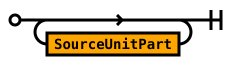
\includegraphics{grammar/sourceunit.jpg}
\caption{SourceUnit}
\end{figure}

\begin{lstlisting}
rule SourceUnit ::=
    SourceUnitPart *  
  ;
\end{lstlisting}

The SourceUnit rule represents the top-level structure of a smart contract source file. It consists of a sequence of source unit parts.

\subsubsection*{Rule SourceUnitPart}

\begin{figure}[!ht]
\centering
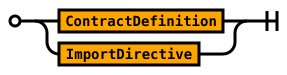
\includegraphics{grammar/sourceunitpart.jpg}
\caption{SourceUnitPart}
\end{figure}

\begin{lstlisting}
rule SourceUnitPart ::=
    ContractDefinition 
  | ImportDirective 
  ;
\end{lstlisting}

The SourceUnitPart rule describes the elements that can appear at the top level of a source file. These elements can be either contract definitions or import directives.

\subsubsection*{Rule ImportDirective}

\begin{figure}[!ht]
\centering
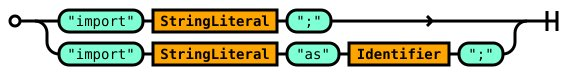
\includegraphics[width=0.8\textwidth]{grammar/importdirective.jpg}
\caption{ImportDirective}
\end{figure}

\begin{lstlisting}
rule ImportDirective ::=
     'import' StringLiteral  ';' 
  |  'import' StringLiteral  'as' Identifier  ';' 
  ;
\end{lstlisting}

The ImportDirective rule defines the syntax for importing other source files into the current file. There are two forms of import directives: a simple import and an import with an alias.

\subsubsection*{Rule Type}

\begin{figure}[!ht]
\centering
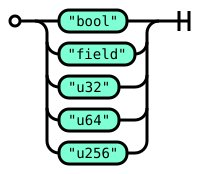
\includegraphics{grammar/type.jpg}
\caption{Type}
\end{figure}

\begin{lstlisting}
rule Type ::=
     'bool' 
  |  'u32' 
  |  'u64' 
  |  'u256' 
  ;
\end{lstlisting}

The Type rule defines the basic types available in the language. These include boolean values (bool),  32-bit unsigned integers (u32), 64-bit unsigned integers (u64), and 256-bit unsigned integers (u256).

\subsubsection*{Rule IdentifierOrError}

\begin{figure}[!ht]
\centering
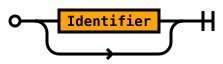
\includegraphics{grammar/identifierorerror.jpg}
\caption{IdentifierOrError}
\end{figure}

\begin{lstlisting}
rule IdentifierOrError ::=
    Identifier 
  | 
  ;
\end{lstlisting}

The IdentifierOrError rule represents either an identifier or an empty element, which can be useful for optional parts of the grammar.

\subsubsection*{Rule VariableDeclaration}

\begin{figure}[!ht]
\centering
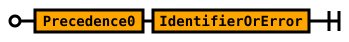
\includegraphics{grammar/variabledeclaration.jpg}
\caption{VariableDeclaration}
\end{figure}

\begin{lstlisting}
rule VariableDeclaration ::=
    Precedence0 IdentifierOrError 
  ;
\end{lstlisting}

The VariableDeclaration rule defines the syntax for declaring a variable. A variable is declared by specifying a type, followed by an optional identifier.

\subsubsection*{Rule StructDefinition}

\begin{figure}[!ht]
\centering
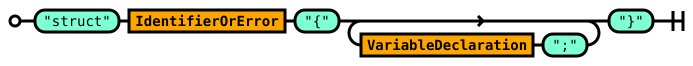
\includegraphics[width=0.8\textwidth]{grammar/structdefinition.jpg}
\caption{StructDefinition}
\end{figure}

\begin{lstlisting}
rule StructDefinition ::=
     'struct' IdentifierOrError  '{' ( VariableDeclaration  ';' ) *   '}' 
  ;
\end{lstlisting}

The StructDefinition rule defines the syntax for declaring a struct type. A struct is a composite data type that groups together variables under a single name.

\subsubsection*{Rule ContractPart}

\begin{figure}[!ht]
\centering
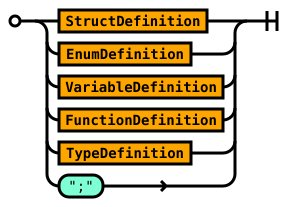
\includegraphics{grammar/contractpart.jpg}
\caption{ContractPart}
\end{figure}

\begin{lstlisting}
rule ContractPart ::=
    StructDefinition 
  | EnumDefinition 
  | VariableDefinition 
  | FunctionDefinition 
  | TypeDefinition 
  |  ';' 
  ;
\end{lstlisting}

The ContractPart rule defines the elements that can appear within a contract definition. These elements include struct definitions, enum definitions, variable definitions, function definitions, and type definitions.

\subsubsection*{Rule ContractDefinition}

\begin{figure}[!ht]
\centering
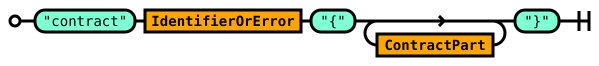
\includegraphics[width=0.8\textwidth]{grammar/contractdefinition.jpg}
\caption{ContractDefinition}
\end{figure}

\begin{lstlisting}
rule ContractDefinition ::=
     'contract' IdentifierOrError  '{' ( ContractPart ) *   '}' 
  ;
\end{lstlisting}

The ContractDefinition rule defines the syntax for declaring a smart contract. A contract is a collection of data and functions that can be executed on a blockchain.

\subsubsection*{Rule EnumDefinition}

\begin{figure}[!ht]
\centering
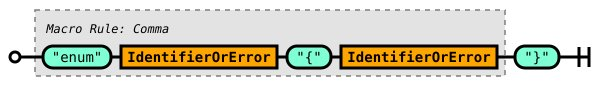
\includegraphics[width=0.8\textwidth]{grammar/enumdefinition.jpg}
\caption{EnumDefinition}
\end{figure}

\begin{lstlisting}
rule EnumDefinition ::=
     'enum' IdentifierOrError  '{' Comma!(IdentifierOrError)  '}' 
  ;
\end{lstlisting}

The EnumDefinition rule defines the syntax for declaring an enumeration type. An enumeration is a data type consisting of a set of named values.

\subsubsection*{Rule VariableDefinition}

\begin{figure}[!ht]
\centering
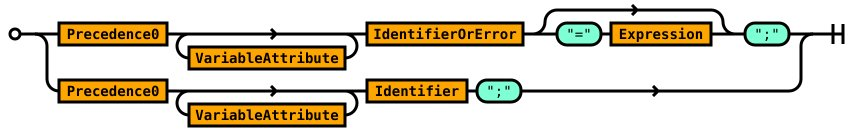
\includegraphics[width=0.8\textwidth]{grammar/variabledefinition.jpg}
\caption{VariableDefinition}
\end{figure}

\begin{lstlisting}
rule VariableDefinition ::=
    Precedence0 VariableAttribute *  IdentifierOrError (  '=' Expression ) ?   ';' 
  | Precedence0 VariableAttribute *  Identifier  ';' 
  ;
\end{lstlisting}

The VariableDefinition rule defines the syntax for defining a variable within a contract. Variables can have attributes such as "const" or "mut" to indicate whether they are constant or mutable.

\subsubsection*{Rule TypeDefinition}

\begin{figure}[!ht]
\centering
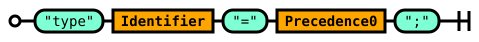
\includegraphics[width=0.8\textwidth]{grammar/typedefinition.jpg}
\caption{TypeDefinition}
\end{figure}

\begin{lstlisting}
rule TypeDefinition ::=
     'type' Identifier  '=' Precedence0  ';' 
  ;
\end{lstlisting}

The TypeDefinition rule defines the syntax for creating a new type alias. A type alias is a way to give a new name to an existing type, which can be useful for improving code readability and maintainability.

\subsubsection*{Rule VariableAttribute}

\begin{figure}[!ht]
\centering
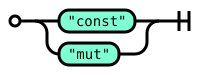
\includegraphics{grammar/variableattribute.jpg}
\caption{VariableAttribute}
\end{figure}

\begin{lstlisting}
rule VariableAttribute ::=
'const'
| 'mut'
;
\end{lstlisting}

The VariableAttribute rule defines the attributes that can be applied to a variable. There are two possible attributes: \verb|const| and \verb|mut|. The \verb|const| attribute indicates that the variable's value cannot be changed after it is initialized, while the \verb|mut| attribute indicates that the variable's value can be modified.

\subsubsection*{Rule Expression}

\begin{figure}[!ht]
\centering
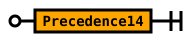
\includegraphics{grammar/expression.jpg}
\caption{Expression}
\end{figure}

\begin{lstlisting}
rule Expression ::=
Precedence14
;
\end{lstlisting}

The Expression rule represents any valid expression in the language. In this case, it refers to the highest level of precedence, Precedence14.

\subsubsection*{Rule Precedence14}

\begin{figure}[!ht]
\centering
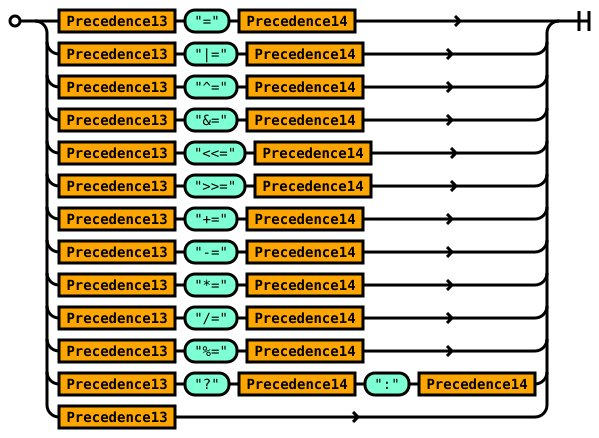
\includegraphics[width=0.8\textwidth]{grammar/precedence14.jpg}
\caption{Precedence14}
\end{figure}

\begin{lstlisting}
rule Precedence14 ::=
Precedence13 '=' Precedence14
| Precedence13 '|=' Precedence14
| Precedence13 '^=' Precedence14
| Precedence13 '&=' Precedence14
| Precedence13 '<<=' Precedence14
| Precedence13 '>>=' Precedence14
| Precedence13 '+=' Precedence14
| Precedence13 '-=' Precedence14
| Precedence13 '*=' Precedence14
| Precedence13 '/=' Precedence14
| Precedence13 '%=' Precedence14
| Precedence13 '?' Precedence14 ':' Precedence14
| Precedence13
;
\end{lstlisting}

The Precedence14 rule defines the various assignment and conditional operators with the highest precedence level. This includes assignment, bitwise OR assignment, bitwise XOR assignment, bitwise AND assignment, left shift assignment, right shift assignment, addition assignment, subtraction assignment, multiplication assignment, division assignment, modulo assignment, and the ternary conditional operator.

\subsubsection*{Rule Precedence13}

\begin{figure}[!ht]
\centering
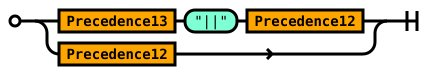
\includegraphics{grammar/precedence13.jpg}
\caption{Precedence13}
\end{figure}

\begin{lstlisting}
rule Precedence13 ::=
Precedence13 '||' Precedence12
| Precedence12
;
\end{lstlisting}

The Precedence13 rule represents the logical OR operator, which has lower precedence than assignment and conditional operators. It allows combining multiple conditions using the ``\verb!||!'' symbol.

\subsubsection*{Rule Precedence12}

\begin{figure}[!ht]
\centering
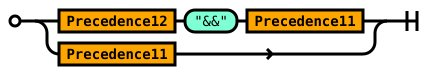
\includegraphics{grammar/precedence12.jpg}
\caption{Precedence12}
\end{figure}

\begin{lstlisting}
rule Precedence12 ::=
Precedence12 '&&' Precedence11
| Precedence11
;
\end{lstlisting}

The Precedence12 rule defines the logical AND operator, which has a lower precedence than the logical OR operator. It is used to combine multiple conditions using the ``\verb|&&|'' symbol.

\subsubsection*{Rule Precedence11}

\begin{figure}[!ht]
\centering
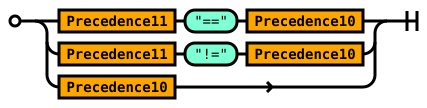
\includegraphics{grammar/precedence11.jpg}
\caption{Precedence11}
\end{figure}

\begin{lstlisting}
rule Precedence11 ::=
    Precedence11  '==' Precedence10 
  | Precedence11  '!=' Precedence10 
  | Precedence10 
  ;
\end{lstlisting}

The Precedence11 rule defines a non-terminal that represents operators with the same precedence level. It has two productions: the first production specifies the equality operator (`\verb|==|') and the next higher precedence non-terminal Precedence10, while the second production specifies the inequality operator (`\verb|!=|') and Precedence10. If neither of these cases applies, Precedence10 is directly considered as the result of this rule. This rule is a useful part of writing a parser or compiler for a programming language, as it can be used to specify operator precedence and associativity.

\subsubsection*{Rule Precedence10}

\begin{figure}[!ht]
\centering
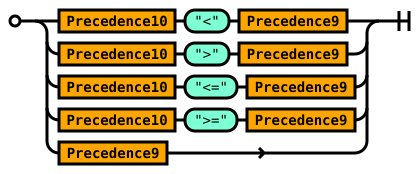
\includegraphics{grammar/precedence10.jpg}
\caption{Precedence10}
\end{figure}

\begin{lstlisting}
rule Precedence10 ::=
    Precedence10  '<' Precedence9 
  | Precedence10  '>' Precedence9 
  | Precedence10  '<=' Precedence9 
  | Precedence10  '>=' Precedence9 
  | Precedence9 
  ;
\end{lstlisting}

The Precedence10 rule defines a non-terminal that represents operators with the same precedence level. It has five productions, each representing a comparison operator (`\verb|<|', `\verb|>|', `\verb|<=|', `\verb|>=|'), followed by the next higher precedence non-terminal Precedence9. If none of these cases apply, Precedence9 is directly considered as the result of this rule. This rule is often used in writing a parser or compiler for a programming language, as it specifies the precedence and associativity of comparison operators.

\subsubsection*{Rule Precedence9}

\begin{figure}[!ht]
\centering
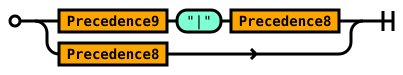
\includegraphics{grammar/precedence9.jpg}
\caption{Precedence9}
\end{figure}

\begin{lstlisting}
rule Precedence9 ::=
    Precedence9  '|' Precedence8 
  | Precedence8 
  ;
\end{lstlisting}

The Precedence9 rule defines a non-terminal that represents operators with the same precedence level. It has two productions: the first production specifies the logical OR operator (`\verb!|!') and the next higher precedence non-terminal Precedence8, while the second production simply specifies Precedence8. If neither of these cases applies, Precedence8 is directly considered as the result of this rule. This rule is often used in writing a parser or compiler for a programming language, as it specifies the precedence and associativity of logical OR operators.

\subsubsection*{Rule Precedence8}

\begin{figure}[!ht]
\centering
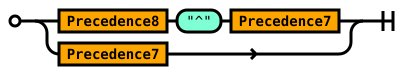
\includegraphics{grammar/precedence8.jpg}
\caption{Precedence8}
\end{figure}

\begin{lstlisting}
rule Precedence8 ::=
    Precedence8  '^' Precedence7 
  | Precedence7 
  ;
\end{lstlisting}

The Precedence8 rule defines a non-terminal that represents operators with the same precedence level. It has two productions: the first production specifies the bitwise XOR operator (`\verb|^|') and the next higher precedence non-terminal Precedence7, while the second production simply specifies Precedence7. If neither of these cases applies, Precedence7 is directly considered as the result of this rule. This rule is often used in writing a parser or compiler for a programming language, as it specifies the precedence and associativity of bitwise XOR operators.

\subsubsection*{Rule Precedence7}

\begin{figure}[!ht]
\centering
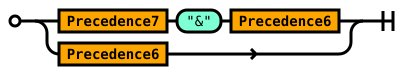
\includegraphics{grammar/precedence7.jpg}
\caption{Precedence7}
\end{figure}

\begin{lstlisting}
rule Precedence7 ::=
    Precedence7  '&' Precedence6 
  | Precedence6 
  ;
\end{lstlisting}

The Precedence7 rule defines a non-terminal that represents operators with the same precedence level. It has two productions: the first production specifies the bitwise AND operator (`\verb|&|') and the next higher precedence non-terminal Precedence6, while the second production simply specifies Precedence6. If neither of these cases applies, Precedence6 is directly considered as the result of this rule. This rule is often used in writing a parser or compiler for a programming language, as it specifies the precedence and associativity of bitwise AND operators.

\subsubsection*{Rule Precedence6}

\begin{figure}[!ht]
\centering
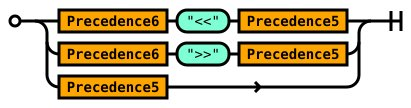
\includegraphics{grammar/precedence6.jpg}
\caption{Precedence6}
\end{figure}

\begin{lstlisting}
rule Precedence6 ::=
    Precedence6  '<<' Precedence5 
  | Precedence6  '>>' Precedence5 
  | Precedence5 
  ;
\end{lstlisting}

The Precedence6 rule defines a non-terminal that represents operators with the same precedence level. It has three productions: the first production specifies the bitwise left shift operator (`\verb|<<|') and the next higher precedence non-terminal Precedence5, the second production specifies the bitwise right shift operator (`\verb|>>|') and Precedence5, while the third production simply specifies Precedence5. If neither of the first two cases applies, Precedence5 is directly considered as the result of this rule. This rule is often used in writing a parser or compiler for a programming language, as it specifies the precedence and associativity of bitwise left shift and bitwise right shift operators.

\subsubsection*{Rule Precedence5}

\begin{figure}[!ht]
\centering
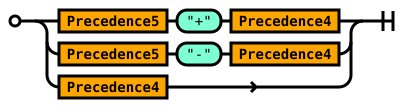
\includegraphics{grammar/precedence5.jpg}
\caption{Precedence5}
\end{figure}

\begin{lstlisting}
rule Precedence5 ::=
    Precedence5  '+' Precedence4 
  | Precedence5  '-' Precedence4 
  | Precedence4 
  ;
\end{lstlisting}

The Precedence5 rule defines a non-terminal that represents operators with the same precedence level. It has three productions: the first production specifies the addition operator (`\verb|+|') and the next higher precedence non-terminal Precedence4, the second production specifies the subtraction operator (`\verb|-|') and Precedence4, while the third production simply specifies Precedence4. If neither of the first two cases applies, Precedence4 is directly considered as the result of this rule. This rule is often used in writing a parser or compiler for a programming language, as it specifies the precedence and associativity of addition and subtraction operators.

\subsubsection*{Rule Precedence4}

\begin{figure}[!ht]
\centering
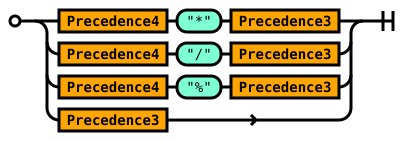
\includegraphics{grammar/precedence4.jpg}
\caption{Precedence4}
\end{figure}

\begin{lstlisting}
rule Precedence4 ::=
    Precedence4  '*' Precedence3 
  | Precedence4  '/' Precedence3 
  | Precedence4  '%' Precedence3 
  | Precedence3 
  ;
\end{lstlisting}

The Precedence4 rule defines a non-terminal that represents operators with the same precedence level. It has four productions: the first production specifies the multiplication operator (`\verb|*|') and the next higher precedence non-terminal Precedence3, the second production specifies the division operator (`'\verb|/|') and Precedence3, the third production specifies the modulus (or remainder) operator (`\verb|%|') and Precedence3, while the fourth production simply specifies Precedence3. If none of the first three cases apply, Precedence3 is directly considered as the result of this rule. This rule is often used in writing a parser or compiler for a programming language, as it specifies the precedence and associativity of multiplication, division, and modulus operators.

\subsubsection*{Rule Precedence3}

\begin{figure}[!ht]
\centering
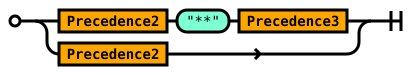
\includegraphics{grammar/precedence3.jpg}
\caption{Precedence3}
\end{figure}

\begin{lstlisting}
rule Precedence3 ::=
    Precedence2  '**' Precedence3 
  | Precedence2 
  ;
\end{lstlisting}



The Precedence3 rule defines a non-terminal that represents operators with the same precedence level. It has two productions: the first production specifies the exponentiation operator (`\verb|**|') and the next higher precedence non-terminal Precedence2, while the second production simply specifies Precedence2. If the first case applies, Precedence3 is considered as the result of the operation Precedence2 raised to the power of Precedence3. Otherwise, Precedence2 is directly considered as the result of this rule. This rule is often used in writing a parser or compiler for a programming language, as it specifies the precedence and associativity of exponentiation operators.

\subsubsection*{Rule Precedence2}

\begin{figure}[!ht]
\centering
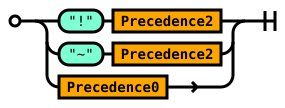
\includegraphics{grammar/precedence2.jpg}
\caption{Precedence2}
\end{figure}

\begin{lstlisting}
rule Precedence2 ::=
     '!' Precedence2 
  |  '~' Precedence2 
  | Precedence0 
  ;
\end{lstlisting}

The Precedence2 rule defines a non-terminal that represents operators with the same precedence level. It has three productions: the first production specifies the logical NOT operator (`\verb|!|') and the same precedence non-terminal Precedence2, the second production specifies the bitwise NOT operator (`\verb|~|') and Precedence2, while the third production simply specifies Precedence0. If either of the first two cases applies, the operator is applied to the result of Precedence2. Otherwise, Precedence0 is directly considered as the result of this rule. This rule is often used in writing a parser or compiler for a programming language, as it specifies the precedence and associativity of logical NOT and bitwise NOT operators.
\subsubsection*{Rule NamedArgument}

\begin{figure}[!ht]
\centering
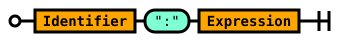
\includegraphics{grammar/namedargument.jpg}
\caption{NamedArgument}
\end{figure}

\begin{lstlisting}
rule NamedArgument ::=
    Identifier  ':' Expression 
  ;
\end{lstlisting}

The NamedArgument rule defines a non-terminal that represents a named argument in a function or method call. It consists of an Identifier followed by a colon and an Expression. The Identifier represents the name of the argument, while the Expression represents its value. This rule is often used in programming languages that support named arguments, allowing for more readable and self-documenting code.

\subsubsection*{Rule FunctionCall}

\begin{figure}[!ht]
\centering
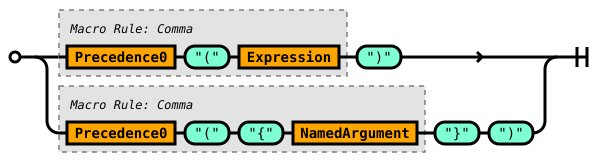
\includegraphics[width=0.8\textwidth]{grammar/functioncall.jpg}
\caption{FunctionCall}
\end{figure}

\begin{lstlisting}
rule FunctionCall ::=
    Precedence0  '(' Comma!(Expression)  ')' 
  | Precedence0  '('  '{' Comma!(NamedArgument)  '}'  ')' 
  ;
\end{lstlisting}

The FunctionCall rule defines a non-terminal that represents a function or method call. It has two productions: the first production specifies an ordered argument list, where the function or method is represented by Precedence0, and the arguments are represented by a comma-separated list of Expression. The second production specifies a named argument list, where the function or method is represented by Precedence0, and the arguments are represented by a comma-separated list of NamedArgument enclosed in braces. This rule is often used in programming languages to represent function or method calls, with the syntax varying depending on the language's support for named arguments and other features.

\subsubsection*{Rule Precedence0}

\begin{figure}[!ht]
\centering
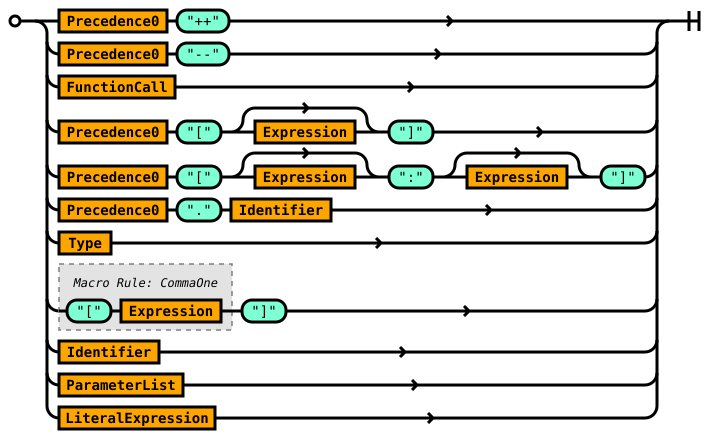
\includegraphics[width=0.8\textwidth]{grammar/precedence0.jpg}
\caption{Precedence0}
\end{figure}

\begin{lstlisting}
rule Precedence0 ::=
    Precedence0  '++' 
  | Precedence0  '--' 
  | FunctionCall 
  | Precedence0  '[' Expression ?   ']' 
  | Precedence0  '[' Expression ?   ':' Expression ?   ']' 
  | Precedence0  '.' Identifier 
  | Type 
  |  '[' CommaOne!(Expression)  ']' 
  | Identifier 
  | ParameterList 
  | LiteralExpression 
  ;
\end{lstlisting}

The Precedence0 rule defines a non-terminal that represents primary expressions, which are the building blocks of more complex expressions. It has multiple productions, including the increment and decrement operators (`\verb|++|' and `\verb|--|'), function or method calls (represented by the non-terminal FunctionCall), array indexing with an Expression inside square brackets, slice notation with two optional Expression separated by a colon inside square brackets, accessing a member of an object using a dot and an Identifier, type names (represented by the non-terminal Type), an array literal with one or more comma-separated Expression enclosed in square brackets, an Identifier, a ParameterList, and a LiteralExpression. These productions specify the most basic elements that can be combined to form more complex expressions in a programming language.

\subsubsection*{Rule LiteralExpression}

\begin{figure}[!ht]
\centering
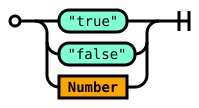
\includegraphics{grammar/literalexpression.jpg}
\caption{LiteralExpression}
\end{figure}

\begin{lstlisting}
rule LiteralExpression ::=
     'true' 
  |  'false' 
  | Number 
  ;
\end{lstlisting}

The LiteralExpression rule defines a non-terminal that represents literal values in a programming language. It has three productions: the first production specifies the Boolean value true, the second production specifies the Boolean value false, and the third production specifies a numeric literal value represented by the non-terminal Number. This rule is often used in programming languages to represent literal values that can be used in expressions, such as Boolean values and numeric constants.

\subsubsection*{Rule Parameter}

\begin{figure}[!ht]
\centering
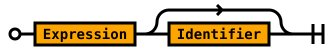
\includegraphics{grammar/parameter.jpg}
\caption{Parameter}
\end{figure}

\begin{lstlisting}
rule Parameter ::=
    Expression Identifier ?  
  ;
\end{lstlisting}

The Parameter rule defines a non-terminal that represents a parameter in a function or method declaration. It consists of an Expression followed by an optional Identifier. The Expression represents the default value of the parameter, while the Identifier represents its name. If the Identifier is not specified, the parameter is treated as an anonymous parameter. This rule is often used in programming languages to define the parameters of functions or methods, allowing the caller to pass arguments to the function or method at runtime.

\subsubsection*{Rule OptParameter}

\begin{figure}[!ht]
\centering
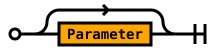
\includegraphics{grammar/optparameter.jpg}
\caption{OptParameter}
\end{figure}

\begin{lstlisting}
rule OptParameter ::=
    Parameter ?  
  ;
\end{lstlisting}

The OptParameter rule defines a non-terminal that represents an optional parameter in a function or method declaration. It consists of an optional Parameter. If the Parameter is present, it specifies a parameter with a default value and an optional name, while if it is absent, there is no default value and no name. This rule is often used in programming languages to provide optional parameters to functions or methods, allowing the caller to omit them if they are not needed.

\subsubsection*{Rule ParameterList}

\begin{figure}[!ht]
\centering
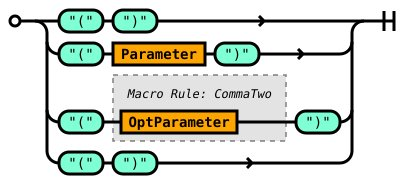
\includegraphics{grammar/parameterlist.jpg}
\caption{ParameterList}
\end{figure}

\begin{lstlisting}
rule ParameterList ::=
     '('  ')' 
  |  '(' Parameter  ')' 
  |  '(' CommaTwo!(OptParameter)  ')' 
  |  '('  ')' 
  ;
\end{lstlisting}

The ParameterList rule defines a non-terminal that represents a list of parameters in a function or method declaration. It has four productions: the first production specifies an empty parameter list, the second production specifies a single parameter, the third production specifies two or more parameters separated by commas, and the fourth production again specifies an empty parameter list. Each parameter is represented by the OptParameter non-terminal, which itself represents an optional parameter with an optional name and default value. This rule is often used in programming languages to define the parameters of functions or methods, allowing the caller to pass arguments to the function or method at runtime.

\subsubsection*{Rule BlockStatementOrSemiColon}

\begin{figure}[!ht]
\centering
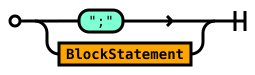
\includegraphics{grammar/blockstatementorsemicolon.jpg}
\caption{BlockStatementOrSemiColon}
\end{figure}

\begin{lstlisting}
rule BlockStatementOrSemiColon ::=
     ';' 
  | BlockStatement 
  ;
\end{lstlisting}

The BlockStatementOrSemiColon rule defines a non-terminal that represents either a semicolon or a block statement in a programming language. It has two productions: the first production specifies a semicolon, and the second production specifies a BlockStatement, which can contain one or more statements enclosed in curly braces. This rule is often used in programming languages to represent the end of a statement or the beginning of a block of statements. If the BlockStatementOrSemiColon is a semicolon, it is typically used to indicate the end of a single statement. If it is a block statement, it is typically used to group multiple statements into a single block that can be executed together.

\subsubsection*{Rule FunctionDefinition}

\begin{figure}[!ht]
\centering
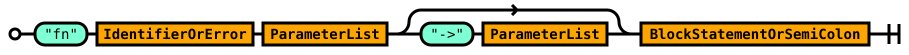
\includegraphics[width=0.8\textwidth]{grammar/functiondefinition.jpg}
\caption{FunctionDefinition}
\end{figure}


\begin{lstlisting}
rule FunctionDefinition ::=
     'fn' IdentifierOrError ParameterList (  '->' ParameterList ) ?  BlockStatementOrSemiColon 
  ;
\end{lstlisting}

The FunctionDefinition rule defines a non-terminal that represents a function definition in a programming language. It consists of the keyword 'fn', followed by an identifier that represents the name of the function, followed by a ParameterList that represents the parameters of the function, and an optional ParameterList that represents the return type of the function. Finally, it ends with a BlockStatementOrSemiColon that represents the body of the function. This rule is often used in programming languages to define functions, which are reusable blocks of code that can be called from other parts of the program. The parameters of the function represent the input values that the function accepts, while the return type represents the output value that the function returns.

\subsubsection*{Rule BlockStatement}

\begin{figure}[!ht]
\centering
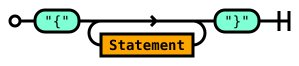
\includegraphics{grammar/blockstatement.jpg}
\caption{BlockStatement}
\end{figure}

\begin{lstlisting}
rule BlockStatement ::=
     '{' Statement *   '}' 
  ;
\end{lstlisting}

The BlockStatement rule defines a non-terminal that represents a block of statements in a programming language. It consists of an opening curly brace, followed by zero or more statements, and finally, a closing curly brace. The statements can be any valid statement in the programming language. This rule is often used in programming languages to group multiple statements together into a single block that can be executed as a unit. A block statement can be used in a variety of contexts, such as in a function body, a loop body, or an if statement body. The block statement allows the programmer to treat multiple statements as a single entity and can be used to make the code more organized and easier to read.

\subsubsection*{Rule OpenStatement}

\begin{figure}
\centering
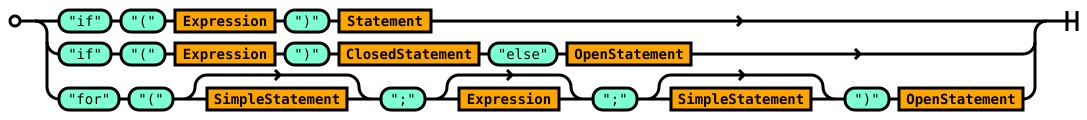
\includegraphics[width=0.8\textwidth]{grammar/openstatement.jpg}
\caption{OpenStatement}
\end{figure}

\begin{lstlisting}
rule OpenStatement ::=
     'if'  '(' Expression  ')' Statement 
  |  'if'  '(' Expression  ')' ClosedStatement  'else' OpenStatement 
  |  'for'  '(' SimpleStatement ?   ';' Expression ?   ';' SimpleStatement ?   ')' OpenStatement 
  ;
\end{lstlisting}

The OpenStatement rule defines a non-terminal that represents an open statement in a programming language. It has three productions: the first production specifies an ``if'' statement with a single statement in its body; the second production specifies an ``if-else'' statement with two sub-statements, one for the ``if'' condition and one for the ``else'' condition; the third production specifies a ``for'' loop with an optional initialization statement, an optional condition, and an optional post-statement, followed by an open statement body. This rule is often used in programming languages to control the flow of execution based on certain conditions or to perform iterative operations on a set of data. The ``if'' statement is used to execute a block of code if a certain condition is true. The ``if-else'' statement is used to execute one of two blocks of code based on whether a certain condition is true or false. The ``for'' loop is used to execute a block of code multiple times while a certain condition is true, and it includes an optional initialization statement, an optional condition, and an optional post-statement.

\subsubsection*{Rule ClosedStatement}

\begin{figure}
\centering
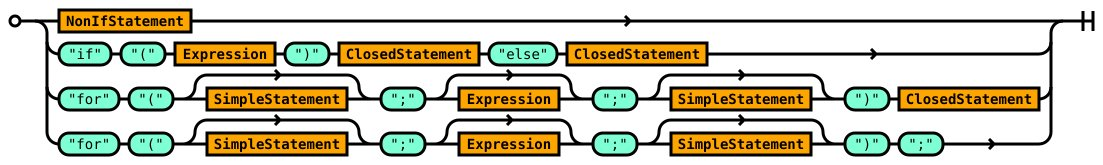
\includegraphics[width=0.8\textwidth]{grammar/closedstatement.jpg}
\caption{ClosedStatement}
\end{figure}

\begin{lstlisting}
rule ClosedStatement ::=
    NonIfStatement 
  |  'if'  '(' Expression  ')' ClosedStatement  'else' ClosedStatement 
  |  'for'  '(' SimpleStatement ?   ';' Expression ?   ';' SimpleStatement ?   ')' ClosedStatement 
  |  'for'  '(' SimpleStatement ?   ';' Expression ?   ';' SimpleStatement ?   ')'  ';' 
  ;
\end{lstlisting}

The ClosedStatement rule defines a non-terminal that represents a closed statement in a programming language. It has four productions: the first production specifies a non-``if'' statements, such as a loop or a function call; the second production specifies an ``if-else'' statement with two sub-statements, both of which are closed statements; the third production specifies a ``for'' loop with an optional initialization statement, an optional condition, and an optional post-statement, followed by a closed statement body; the fourth production specifies a ``for'' loop with an optional initialization statement, an optional condition, and an optional post-statement, followed by a semicolon. This rule is often used in programming languages to control the flow of execution based on certain conditions or to perform iterative operations on a set of data. The closed statement differs from the open statement in that it contains a complete sub-statement within its body.

\subsubsection*{Rule Statement}

\begin{figure}
\centering
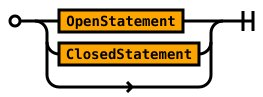
\includegraphics{grammar/statement.jpg}
\caption{Statement}
\end{figure}

\begin{lstlisting}
rule Statement ::=
    OpenStatement 
  | ClosedStatement 
  | 
  ;
\end{lstlisting}

This rule is used to define the structure of statements in a programming language. Statements are used to express an action that needs to be carried out, such as assigning a value to a variable or looping over a set of data. The Statement rule is often used in the context of defining control structures like loops and conditionals.

\subsubsection*{Rule SimpleStatement}

\begin{figure}
  \centering
  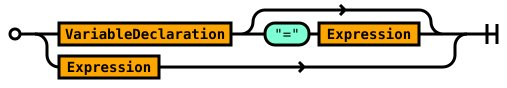
\includegraphics[width=0.8\textwidth]{grammar/simplestatement.jpg}
  \caption{SimpleStatement}
  \end{figure}

\begin{lstlisting}
rule SimpleStatement ::=
    VariableDeclaration (  '=' Expression ) ?  
  | Expression 
  ;
\end{lstlisting}

The SimpleStatement rule is used to define a simple statement in a programming language. It has two possible productions. The first production specifies a VariableDeclaration, which may or may not be followed by an \verb|=| sign and an Expression. This allows for the declaration of a variable with an optional initial value. The second production specifies an Expression, which is a piece of code that evaluates to a value.

\subsubsection*{Rule NonIfStatement}

\begin{figure}
  \centering
  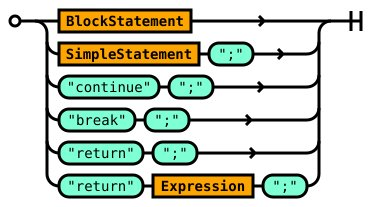
\includegraphics{grammar/nonifstatement.jpg}
  \caption{NonIfStatement}
  \end{figure}

\begin{lstlisting}
rule NonIfStatement ::=
    BlockStatement 
  | SimpleStatement  ';' 
  |  'continue'  ';' 
  |  'break'  ';' 
  |  'return'  ';' 
  |  'return' Expression  ';' 
  ;
\end{lstlisting}

The NonIfStatement rule is used to define a non-conditional statement in a programming language. It has several possible productions, including a BlockStatement and a SimpleStatement followed by a semicolon.

The BlockStatement production allows for a block of code to be executed as a single unit and is often used to group multiple statements. The SimpleStatement followed by a semicolon production allows for a single statement to be executed.

In addition, the rule specifies three special types of statements: continue, break, and return. The continue statement is used to skip to the next iteration of a loop, while the break statement is used to exit a loop. The return statement is used to exit a function and optionally return a value.

Overall, the NonIfStatement rule is an important part of defining the syntax of a programming language and is used to express a wide range of statements and behaviors.

\subsubsection*{Macro Comma}

\begin{figure}
  \centering
  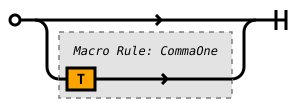
\includegraphics{grammar/comma.jpg}
  \caption{Comma}
  \end{figure}

\begin{lstlisting}
macro Comma<T> ::=
    
  | CommaOne!(T) 
  ;
\end{lstlisting}

This is a macro definition for a comma-separated list of elements of type T. It allows for zero or more elements separated by commas. The \verb|!| symbol after the macro name indicates that the macro is left-recursive, meaning it can be applied repeatedly until it no longer matches. The \verb|CommaOne!| in the definition means that the macro should match at least one element before the optional commas.

\subsubsection*{Macro CommaOne}

\begin{figure}
  \centering
  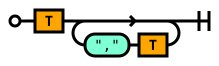
\includegraphics{grammar/commaone.jpg}
  \caption{CommaOne}
  \end{figure}

\begin{lstlisting}
macro CommaOne<T> ::=
    T (  ',' T ) *  
  ;
\end{lstlisting}

This is a macro definition for a comma-separated list of one or more elements of type \verb|T|. It first matches a single element of type \verb|T|, followed by zero or more occurrences of a comma followed by another element of type \verb|T|. The \verb|*| after the second parentheses indicates that this sequence can repeat zero or more times. This macro enforces that there must be at least one element in the comma-separated list.

\subsubsection*{Macro CommaTwo}

\begin{figure}
  \centering
  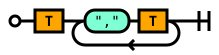
\includegraphics{grammar/commatwo.jpg}
  \caption{CommaTwo}
  \end{figure}

\begin{lstlisting}
macro CommaTwo<T> ::=
    T (  ',' T ) +  
  ;
\end{lstlisting}

The CommaTwo macro is used to match one or more occurrences of the same non-terminal symbol separated by commas.

\subsubsection*{Rule Number}

\begin{figure}
  \centering
  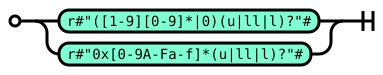
\includegraphics{grammar/number.jpg}
  \caption{Number}
  \end{figure}

\begin{lstlisting}
rule Number ::=
     'r#([1-9][0-9]*|0)#' 
  |  'r#0x[0-9A-Fa-f]*#' 
  ;
\end{lstlisting}

The Number rule is used to define a number in a programming language. It has two possible productions. The first production matches a decimal number, while the second production matches a hexadecimal number.

\subsubsection*{Rule Identifier}

\begin{figure}
  \centering
  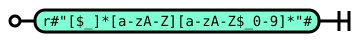
\includegraphics{grammar/identifier.jpg}
  \caption{Identifier}
  \end{figure}

\begin{lstlisting}
rule Identifier ::=
'r#[$_][a-zA-Z][a-zA-Z$_0-9]#'
;
\end{lstlisting}

The Identifier rule is used to define an identifier in a programming language. It matches a sequence of characters that starts with a letter or underscore, followed by zero or more letters, numbers, underscores, or dollar signs.

\subsubsection*{Rule StringLiteral}

\begin{figure}
  \centering
  \includegraphics{grammar/stringliteral.jpg}
  \caption{StringLiteral}
  \end{figure}

\begin{lstlisting}
rule StringLiteral ::=
'r#\[^\]*\#'
;
\end{lstlisting}

The StringLiteral rule is used to define a string literal in a programming language. It matches a sequence of characters surrounded by square brackets.

\subsection{Smart Contracts}


Ola contracts allow users to write complex business logic that will be deployed to Ola's L2 network, and cross-contract calls can be written between different contracts just like solidity.

\subsubsection{Simple Examples}

The following example shows a recursive and non-recursive Ola smart contract implementation of Fibonacci numbers.

\begin{lstlisting}
contract Fibonacci {

    fn main() {
       fib_non_recursive(10);
    }

    fn fib_recursive(u32 n) -> (u32) {
        if (n == 0 || n == 1) {
            return 1;
        }
        return fib_recursive(n -1) + fib_recursive(n -2);
    }

    fn fib_non_recursive(u32 n) -> (u32) {
        u32 first = 0;
        u32 second = 1;
        u32 third = 1;
        for (u32 i = 2; i <= n; i++) {
             third = first + second;
             first = second;
             second = third;
        }
        return third;
    }

}
\end{lstlisting}

The following shows a simple Person contract that contains a person structure, assigns a value to the Person structure, and reads the status of the person.

\begin{lstlisting}
contract Person {

    enum Sex {
        Man,
        Women
    }

    struct Person {
        Sex s;
        u32 age;
        u256 id;
    }

    Person p;

    fn newPerson(Sex s, u32 age, u256 id) {
        p = Person(s, age, id);
    }

    fn getPersonId() -> (u256) {
        return p.id;
    }

    fn getAge() -> (u32) {
        return p.age;
    }
}
\end{lstlisting}

\subsubsection{Multiple files}

For better project organization and clearer logic, it is common to split the contents of a file into multiple files. Ola language supports the import of another contract within a contract through the `import` keyword.

An example of a multi-file contract is shown below.

\textbf{Contract RectangularCalculator}

\begin{lstlisting}
contract RectangularCalculator {
  
    fn rectangle(u32 w, u32 h) -> (u32 s, u32 p) {
        s = w * h;
        p = 2 * (w + h);
        // Returns a variable with the same name, the return can be ignored
        //return (s, p)
    }
}
\end{lstlisting}

\textbf{Contract ShapeCalculator}

\begin{lstlisting}
contract SquareCalculator {

    fn square(u32 w) -> (u32 s, u32 p) {
        s = w * w;
        p = 4 * w;
        return (s, p);
    }
}
\end{lstlisting}

\textbf{Contract Calculator}

\begin{lstlisting}
import "./RectangularCalculator";
import "./SquareCalculator";

contract Calculator {
  
    fn sum(u32 w, u32 h) -> (u32 s, u32 p) {
        (u32 rectangle_s, u32  rectangle_p) = rectangle(w, h);
        (u32 square_s, u32 square_p) = square(w);
        return (rectangle_s + square_s, rectangle_p + square_p);
    }
}
\end{lstlisting}


\subsection{Ola Compiler}

\subsubsection{Ola Compiler Introduction}

The Ola-lang compiler compiles the high-level Ola contract code into OlaAsm assembly code supported by OlaVM. 

The general pipeline process is as follows:

\begin{figure}[!htp]
    \centering
    \includegraphics[width=0.6\textwidth]{ola-lang-intro.jpg}
    \caption{Ola-lang pipeline}
    \label{fig:ola-lang-intro}
\end{figure}
program->ir process and structure detailed diagram (expand below)

Structure:

    Tokens

    Ast

    IR

IR process

Devices:

    Lex and Syntax

    Semantics

    IR generation
\subsubsection{Ola Compiler Backend}

Detailed diagram of ir->asm flow and structure (expanded below)

Structure:

    lists

    insts

    mcinsts

ABI:

    Function call specification

    Mapping Relationships to Virtual Memory

Devices:

    IR parsing

    Target code generation

        Function call demotion

        Instruction selection

        Register Allocation

        Slot elimination

        Stack frame handling

        Assembly printing

    \begin{itemize}
        \item IR parsing

    IR is composed of the following structure: module -> function -> value -> types.

    Module structure contains Target (triple and datalayout information), Function, Attribute, GlobalVariable.

    Function structure contains name, type information, Visibility, Attribute and Parameter list basic information, and data, Layout.

    Among them, layout contains the sequential logical relationship between basicBlocks and the instructions within them.

    Data contains the specific Value, Instruction, BasicBlock list instances.

    BasicBlock is identified by BasicBlockId and consists of two parts: name and number. Each BB block usually contains one preds and one sucs.

    Instruction is identified by BasicBlockId+InstructionId and usually consists of Opcode, Operand, dest and the Type of its operation.

    Value contains Instruction, Argument, Constant and InlineAsm types.

    Due to the characteristics of the instruction set of olavm, the type is currently mainly i64 type.

        \item IR parsing process

        process: targetDatalayout/targetTriple -> attributeGroup -> localType -> globalVariable -> function -> metadata.

    The function is mainly divided into two parts: parseArgumentList and parseBody.

        \item IR opt pass

    Pre-analysis analysis pass is mainly DominatorTree, conversion transform pass contains dce, mem2reg, sccp.

        \item back-end codegen modules

    bridging ir structure of module, function, and isa related callconv, register and isa, code generation related lower and optimization related pass.

    TargetISA main contains custom TargetInst, Register(RegisterClass/RegisterInfo), lower and modulepasses, callconv, datalayout information.

    Module in addition to inheritance Ir parsed out Module, the description of its Function and ir differ significantly.

    Data information: BasicBlock in the instructions for Target Instruction, register contains VRegs and RegUnit two categories, and contains a vregtoinsts mapping.
    At the same time, Inst in Layout are referred to TargetInst.
    Note that the memory access operations of parameters, local variables, etc. are described by the structure of slot(ptr+offset).

    The lower module provides the process of downgrading LoweringContext to Instruction, and for function calls it also requires copyargstovregs.

    The pass module contains the regalloc and spiller for analyzing the liveness of the pass and the function pass.

        \item back-end process

    Register and insts description

    Function call demotion

    Instruction selection

    eliminateslot

    proepiinserter

    reg allocation and coalescing
    
    \end{itemize}
\subsubsection{Lib funtions}





    \printbibliography[heading=bibintoc, title=\ebibname]
\end{document}
